\documentclass{standalone}

\usepackage{tikz}

\begin{document}

\begin{tikzpicture}

\node at (0, 0) {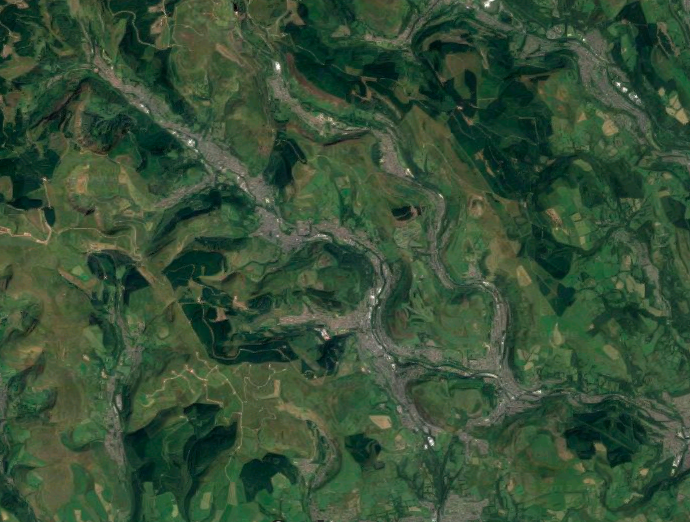
\includegraphics{rhondda}};

\node[circle, draw=yellow, fill=yellow] (porth) at (6, -4) {}; % Porth
\node[circle, draw=yellow, fill=yellow] (tonypandy) at (1, -3) {}; % Tonypandy
\node[circle, draw=yellow, fill=yellow] (penygraig) at (2, -4.5) {}; % Penygraig
\node[circle, draw=yellow, fill=yellow] (llwynypia) at (1.5, -1) {}; % Llwynypia
\node[circle, draw=yellow, fill=yellow] (wattstown) at (5, -0.5) {}; % Wattstown
\node[circle, draw=yellow, fill=yellow] (maerdy) at (-2, 6) {}; % Maerdy
\node[circle, draw=yellow, fill=yellow] (ystrad) at (0, 1) {}; % Ystrad
\node[circle, draw=yellow, fill=yellow] (penrhys) at (2.5, 1) {}; % Penrhys
\node[circle, draw=yellow, fill=yellow] (treorchy) at (-4, 3.5) {}; % Treorchy
\node[circle, draw=yellow, fill=yellow] (treherbert) at (-7.5, 6) {}; % Treherbert

\node[fill=none, draw=none, text=yellow] at ($(porth) - (0.5, 0.5)$) {\Large{Porth}};
\node[fill=none, draw=none, text=yellow] at ($(tonypandy) - (0.5, 0.5)$) {\Large{Tonypandy}};
\node[fill=none, draw=none, text=yellow] at ($(penygraig) - (0.5, 0.5)$) {\Large{Penygraig}};
\node[fill=none, draw=none, text=yellow] at ($(llwynypia) - (0.5, 0.5)$) {\Large{Llwynypia}};
\node[fill=none, draw=none, text=yellow] at ($(wattstown) - (0.5, 0.5)$) {\Large{Wattstown}};
\node[fill=none, draw=none, text=yellow] at ($(maerdy) - (0.5, 0.5)$) {\Large{Maerdy}};
\node[fill=none, draw=none, text=yellow] at ($(ystrad) - (0.5, 0.5)$) {\Large{Ystrad}};
\node[fill=none, draw=none, text=yellow] at ($(penrhys) - (0.5, 0.5)$) {\Large{Penrhys}};
\node[fill=none, draw=none, text=yellow] at ($(treorchy) - (0.5, 0.5)$) {\Large{Treorchy}};
\node[fill=none, draw=none, text=yellow] at ($(treherbert) - (0.5, 0.5)$) {\Large{Treherbert}};

\end{tikzpicture}

\end{document}
